%---------------------------------------------------------------------------%
%-                                                                         -%
%-                           LaTeX Template                                -%
%-                                                                         -%
%---------------------------------------------------------------------------%
%- Copyright (C) Huangrui Mo <huangrui.mo@gmail.com> 
%- This is free software: you can redistribute it and/or modify it
%- under the terms of the GNU General Public License as published by
%- the Free Software Foundation, either version 3 of the License, or
%- (at your option) any later version.
%---------------------------------------------------------------------------%
%->> Document class declaration
%---------------------------------------------------------------------------%
\documentclass{Style/ucasproposal}%
%- Multiple optional arguments:
%- [<oneside|twoside|print>]% oneside eprint, twoside eprint, or paper print
%- [fontset=<adobe|none|...>]% specify font set instead of automatic detection
%- [scheme=plain]% thesis writing of international students
%- [draftversion]% show draft version information
%- [standard options for ctex article class: draft|paper size|font size|...]%
%---------------------------------------------------------------------------%
%->> Document settings
%---------------------------------------------------------------------------%
\usepackage[numbers,list,xhf]{Style/artratex}% document settings
%- usage: \usepackage[option1,option2,...,optionN]{artratex}
%- Multiple optional arguments:
%- [bibtex|biber]% set bibliography processor and package
%- [<numbers|super|authoryear|alpha>]% set citation and reference style
%- <numbers>: textual: Jones [1]; parenthetical: [1]
%- <super>: textual: Jones superscript [1]; parenthetical: superscript [1]
%- <authoryear>: textual: Jones (1995); parenthetical: (Jones, 1995)
%- <alpha>: textual: not available; parenthetical: [Jon95]
%- [geometry]% reconfigure page layout via geometry package
%- [lscape]% provide landscape layout environment
%- [xhf]% disable header and footer via fancyhdr package
%- [color]% provide color support via xcolor package
%- [background]% enable page background
%- [tikz]% provide complex diagrams via tikz package
%- [table]% provide complex tables via ctable package
%- [list]% provide enhanced list environments for algorithm and coding
%- [math]% enable some extra math packages
%- [xlink]% disable link colors
\usepackage{Style/artracom}% user defined commands
%---------------------------------------------------------------------------%
%->> Document inclusion
%---------------------------------------------------------------------------%
%\includeonly{Tex/Chap_1,...,Tex/Chap_N}% selected files compilation
%---------------------------------------------------------------------------%
%->> Document content
%---------------------------------------------------------------------------%
%-
%-> Titlepage information
%-
%-> 中文封面信息
%-
\schoollogo{scale=0.112}{ucas_logo}% 校徽
\title{多架构软硬协同二进制翻译的实现和优化}% 题目
\author{晏悦}% 作者姓名
\authorid{202128013229037}% 学号
\advisor{王剑}% 指导老师
\advisortitle{研究员}% 指导老师职务
\degree{硕士}% 学位:硕士、博士
\degreetype{工学}% 学位类别:理学、工学、工程、医学等
\major{计算机系统结构}% 二级学科专业名称
\field{体系结构}% 研究方向
\institute{中国科学院计算技术研究所}% 院所
%\institute{中国科学院力学研究所\\流固耦合实验室}% 多行院所名称示例
%\chinesedate{2014~年~06~月}% 日期
%---------------------------------------------------------------------------%
\begin{document}
%-
%-> Frontmatter: title page, abstract, content list, symbol list, preface
%-
\pagenumbering{roman}% page numbers with roman style
% \input{Tex/Frontmatter}% title page, abstract

%---------------------------------------------------------------------------%
%-> Frontmatter
%---------------------------------------------------------------------------%
%-
%-> 生成封面
%-
\maketitle% 生成中文封面
%-
%-> 目录
%-
\tableofcontents% 生成目录
%---------------------------------------------------------------------------%
%-
%-> Mainmatter
%-
\clearpage
\pagenumbering{arabic}% restart page numbers with arabic style
% %---------------------------------------------------------------------------%
%->> Main content
%---------------------------------------------------------------------------%
\section{选题的背景及意义}

\subsection{选题背景}

关于riscv生态,以及各类指令集生态的问题。

阐述二进制翻译器的问题,以及二进制翻译器的优势。



\subsubsection{背景}


\subsection{选题意义}



\subsubsection{意义}



\section{国内外本学科领域的发展现状与趋势}



\section{课题主要研究内容、预期目标}



\section{拟采用的研究方法、技术路线、实验方案及其可行性分析}



\section{已有科研基础与所需的科研条件}



\section{研究工作计划与进度安排}



\section*{填表说明}

本表内容须真实、完整、准确。

\section*{常见使用问题}

\begin{enumerate}
    \item 模板使用说明请见 \href{https://github.com/mohuangrui/ucasthesis}{ucasthesis:中国科学院大学学位论文 LaTeX 模板}.
    \item 填表说明和模板说明不是开题报告的一部分,请删除。
    \item 开题报告样式设计导致对题目换行与不换行难以兼容,排版十分困难。推荐采用当前设置,尽量避免将精力花在这些无关紧要的细节上。
\end{enumerate}

\nocite{*}% 使文献列表显示所有参考文献(包括未引用文献)
%---------------------------------------------------------------------------%
% main content
%---------------------------------------------------------------------------%
%->> Main content
%---------------------------------------------------------------------------%

%---------------------------------------------------------------------------%
%->> Chapter 1
%---------------------------------------------------------------------------%
\section{选题的背景及意义}

随着计算机技术的发展,各种指令集架构层出不穷,如X86、ARM、LoongArch\cite{LoongArch2023}、RISCV等。这些指令集之间互不兼容,导致软件需要针对不同架构进行多次开发和编译,无法进行通用迁移,增加了软件开发的成本和复杂度。

\subsection{中国国产CPU的多样性}

% https://zhuanlan.zhihu.com/p/599483286 国产CPU的发展现状
中国国产CPU在多个架构上展现出丰富多彩的发展,其中X86、ARM、LoongArch和RISCV等架构代表了不同的技术路线,由各个公司推动。参见表\ref{tab:CPUs},以下是各架构的特点:

% https://www.tablesgenerator.com/latex_tables 生成latex表格
\begin{table}[]
\centering
\caption{国产CPU的发展现状}
\label{tab:CPUs}
    \begin{tabular}{llll}
    \rowcolor[HTML]{FBE5D6} 
    指令集       & 代表公司   & 优势        & 不足         \\
    X86       & 兆芯,海光  & 兼容Windows & 授权问题 \\
    ARM       & 华为,飞腾  & 兼容安卓      & 授权问题       \\
    LoongArch & 龙芯     & 自主可控      & 生态不足       \\
    RISCV     & 开芯院,阿里 & 开源开放      & 生态不足      
    \end{tabular}
    \end{table}


    \begin{itemize}
    \item {X86架构: } 代表公司为兆芯和海光,采用X86架构IP内核授权模式,可基于公版CPU核进行优化或修改,性能起点高,生态壁垒相对低。但是依赖海外企业授权,自主可控风险偏高。
    
    \item{ARM架构:} 代表公司为华为和飞腾,采用Armv8永久授权,具有更高的自主化程度,可自行研发设计CPU内核和芯片,也可扩充指令集。但是存在长期隐患,因为Arm将不再向这些国产CPU厂商提供Armv9的永久授权。
    
    \item{LoongArch架构:} 代表公司为龙芯,采用LoongArch指令集,具有相对更高的自主可控程度,已经在国产军工行业得到了广泛应用。但是生态不足,需要大量投入才能建立起完善的软件生态。
    
    \item{RISCV架构:} 代表公司为开源芯片研究院和阿里平头哥,采用RISCV架构,具有相对精简的指令集架构(ISA),并遵循开源宽松的BSD协议,在国内得到了迅速发展,但同样生态不足。
    \end{itemize}


\subsection{指令集生态的碎片化与兼容性问题}

\begin{figure}[h]
    \centering
    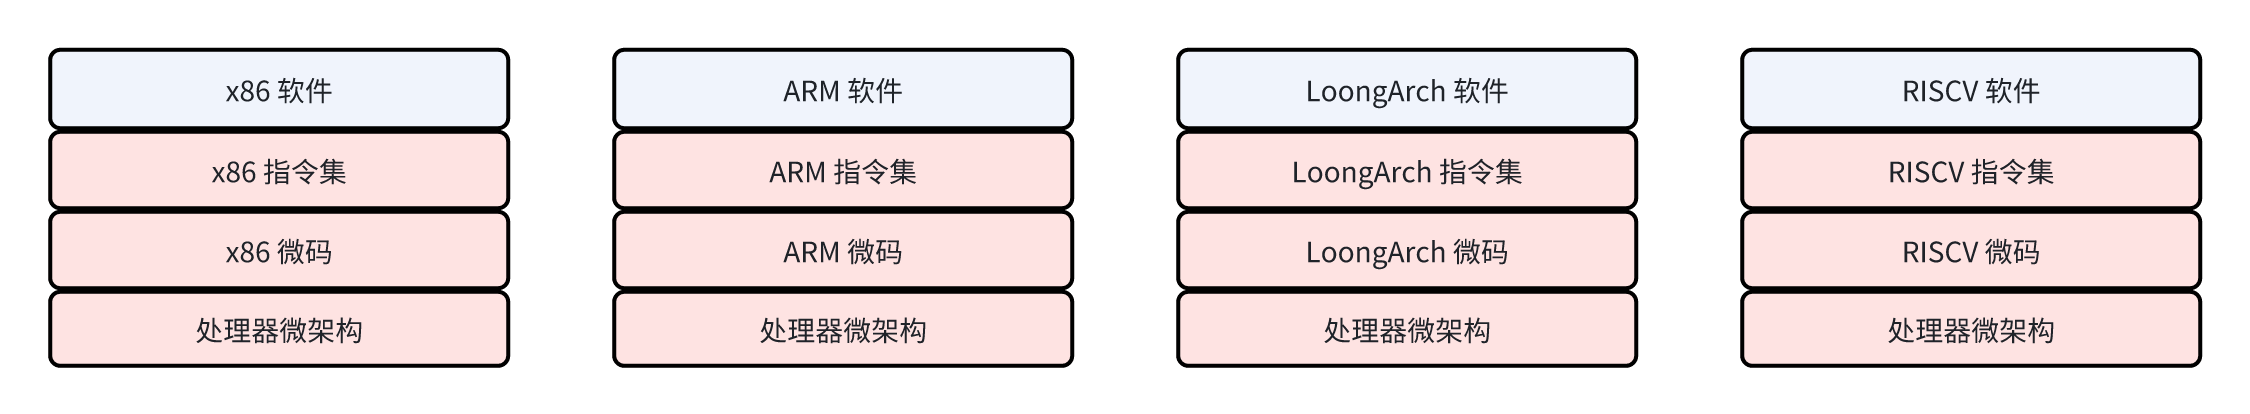
\includegraphics[width=1\linewidth]{./feishuImage/allCPU_arch.png}
    \caption{不同指令集CPU的架构图,图中白色为软件层,红色为硬件层,并忽略了操作系统,这不是本文研究重点。\protect\footnotemark}
    \label{img:allCPU_arch}
  \end{figure}

\footnotetext{ARM, LoongArch, RISCV 等精简指令集架构(RISC)的CPU,内部可以实现微码层,也可以不实现,根据具体CPU微架构实现而不同。}

如图\ref{img:allCPU_arch}所示,同一套软件源代码需要针对不同的指令集进行编译才能在不同架构的CPU上运行。

    而中国国产CPU的多样性导致了指令集的碎片化,增加了应用程序在不同架构间迁移和适配的复杂性。存在的问题包括:
    \begin{itemize}
    \item \textbf{适配和迁移负担:} 不同架构间的适配和迁移需要大量人力和物力资源。
    
    \item \textbf{历史兼容包袱:} 不同指令集的历史兼容包袱使得跨架构的兼容性复杂。
    
    \item \textbf{编译与源代码的限制:} 古老软件无源代码,只能通过翻译运行以适应新的指令集。
    
    \item \textbf{操作系统支持的挑战:} 操作系统厂商需要投入更多资源以支持不同架构。
    \end{itemize}

\subsection{二进制翻译技术的重要性}
目前,二进制翻译技术是解决指令集兼容性问题的主要方法。

\begin{figure}[h]
    \centering
    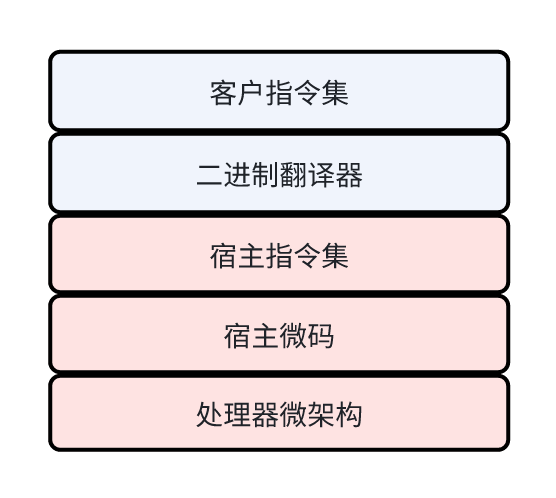
\includegraphics[width=0.3\linewidth]{./feishuImage/BT_arch.png}
    \caption{二进制翻译器架构图,能在宿主指令集机器上运行客户程序。}
    \label{img:BT_arch}
  \end{figure}

如图\ref{img:BT_arch} 二进制翻译技术能够将一个指令集(称为客户指令集)上的二进制程序翻译到另一种指令集(称为宿主指令集)上执行,分为系统级和用户级二进制翻译。系统级翻译涉及整个操作系统,而用户级翻译主要处理用户程序。用户级翻译由于不需要模拟特权态和物理内存,因此性能更高,在软件生态迁移中更为常见,在后文中提及的二进制翻译器默认为用户级二进制翻译器。

\subsection{二进制翻译器性能问题}
现有的开源二进制翻译器性能
\footnote{
    目前工业界和学术界对二进制翻译的性能有着默认统一的定义:同一份测试程序的源码用相同编译参数,编译到客户指令集和宿主指令集,得到两份二进制文件$B_g$和$B_h$。
    在硬件平台用二进制翻译运行客户程序$B_g$的时间记为$T_{bt}$,在同一硬件平台直接运行宿主程序$B_h$的时间记为$T_h$。
    二进制翻译的性能则为翻译运行时间除以原生运行时间$\frac{T_{bt}}{T_h}$。
}
相对较低,例如QEMU\cite{bellardQEMUFastPortable2005}虽然支持多架构应用,但在翻译运行SPEC CPU 2017\cite{SPECCPU2017}程序时候,仅有约10\%的性能。商业二进制翻译器也存在性能损失,
如苹果的Rosetta2\cite{RosettaTranslationEnvironment, RunningIntelBinaries}、
华为的ExaGear\cite{KunPengExaGear}、
和龙芯的LATX\cite{LoongArchEnv2022, LoongArch2023},
性能仅达到原生运行的70\%左右,并且仅能保证单一指令集翻译到单一指令集,并不通用,多架构支持较为困难。这直接影响了软件生态迁移的流畅度和成功性。

\subsection{多架构软硬协同二进制翻译的需求}

为了解决\textbf{指令集碎片化}和\textbf{二进制翻译器性能}问题,迫切需要多架构软硬协同的二进制翻译技术。这项技术的关键目标是在同一套硬件下实现多指令集的共存,为软件提供更好的跨平台兼容性和性能表现。

这种技术的优势在于:

1. \textbf{打破指令集边界,消除应用迁移成本:} 应用程序无需适配和迁移至特定指令集,可直接在同一套硬件上运行,降低了软件开发和维护的复杂性。

2. \textbf{硬件对外暴露微码,规避X86等授权问题:} 通过在硬件层面暴露微码,技术在一定程度上规避了X86等架构的授权问题,提高了国产CPU的自主性。

3. \textbf{软件维护历史兼容,微码迭代优化:} 作为软件层面的核心组件,二进制翻译器维护历史兼容性并实现微码迭代优化,确保不同架构的硬件在不同历史时期的应用中保持高效运行。

如图\ref{img:my_arch}所示,本文提出了一种多架构软硬协同的二进制翻译技术,通过在硬件层面支持一套融合微码,为软件层面的二进制翻译器提供更好的性能和兼容性。这项技术可降低软件开发和维护的复杂性,弥合不同指令集的生态差异,对中国国产CPU的发展具有重要意义。


\begin{figure}[h]
    \centering
    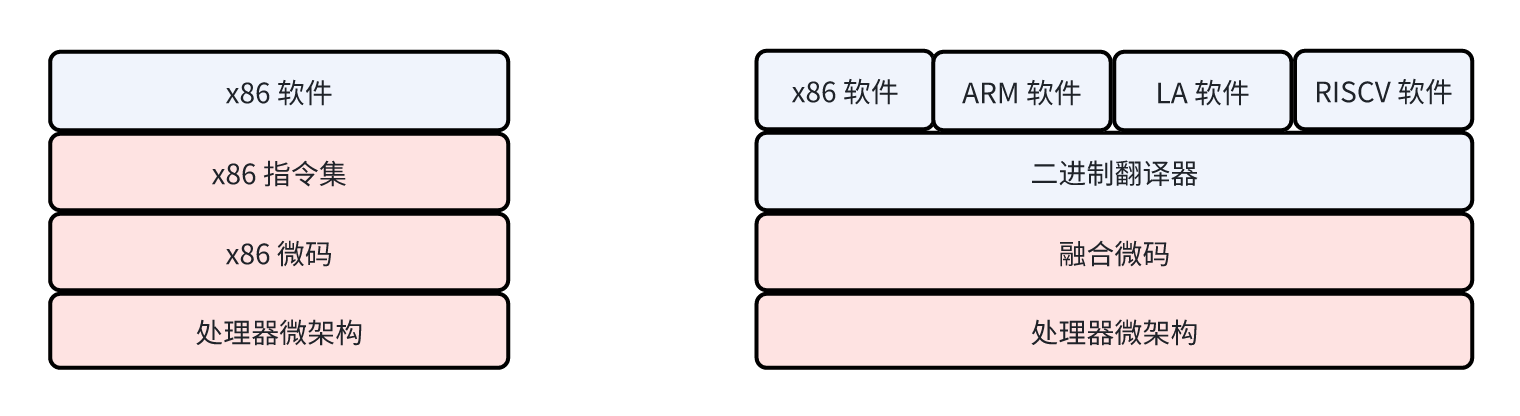
\includegraphics[width=1\linewidth]{./feishuImage/my_arch.png}
    \caption{多架构软硬协同的二进制翻译架构图,硬件仅对外暴露微码,软件层面的二进制翻译器可以实现多架构的支持,性能接近原生运行性能。}
    \label{img:my_arch}
  \end{figure}


%---------------------------------------------------------------------------%
%->> Chapter 2
%---------------------------------------------------------------------------%

\section{国内外本学科领域的发展现状与趋势}
% \section{国内外相关工作}

\subsection{全美达公司的工作}

全美达公司在过去的几十年中在低功耗、兼容X86架构的微处理器领域取得了显著的成就。其代表性产品 Crusoe 系列微处理器于 2000 年首次推出,引起了业界的广泛关注。

全美达的工作重点是开发基于超长指令字(VLIW)处理器的微处理器,并结合软件侧的代码转换器,以实现低功耗、兼容X86的微处理器。

\subsubsection{代码转换器架构}

全美达的代码转换器\cite{dehnertTransmetaCodeMorphing2003}由解释器、运行时系统和动态二进制翻译器组成。在执行程序时,X86指令首先通过解释器进行解释执行并进行分析。根据代码块的执行频率,动态二进制翻译器逐步生成更优化的翻译,并将不同的指令组合成一条超长指令,指向底层硬件。这种方法类似于目前主流的多发射处理器的工作原理,在一拍内同时运行多条指令,通过动态地生成优化的超长指令来提高执行效率。

\subsubsection{Crusoe 微处理器}

全美达Crusoe 微处理器系列是该公司推出的兼容X86的微处理器,于 2000 年首次亮相。其中 Crusoe 以其实现 X86 兼容性的独特方式而著称。

Crusoe 运行的是一种称为代码转换器的软件抽象层或虚拟机,而不是在硬件中实现或由专用硬件进行转换的指令集架构。如图\ref{img:transmeta_arch}所示,代码转换器将从程序接收到的X86汇编代码指令翻译成微处理器的本机指令(超长指令字)。通过这种方式,Crusoe 也可以模拟其他指令集架构,例如Crusoe 也能将字节码翻译为其本机指令集中的指令来执行 Java 字节码。

这种架构的优势在于,通过在 X86 指令流和硬件之间引入抽象层,只需修改代码转换器,就可以在不破坏兼容性的情况下更改硬件架构。

\begin{figure}[h]
    \centering
    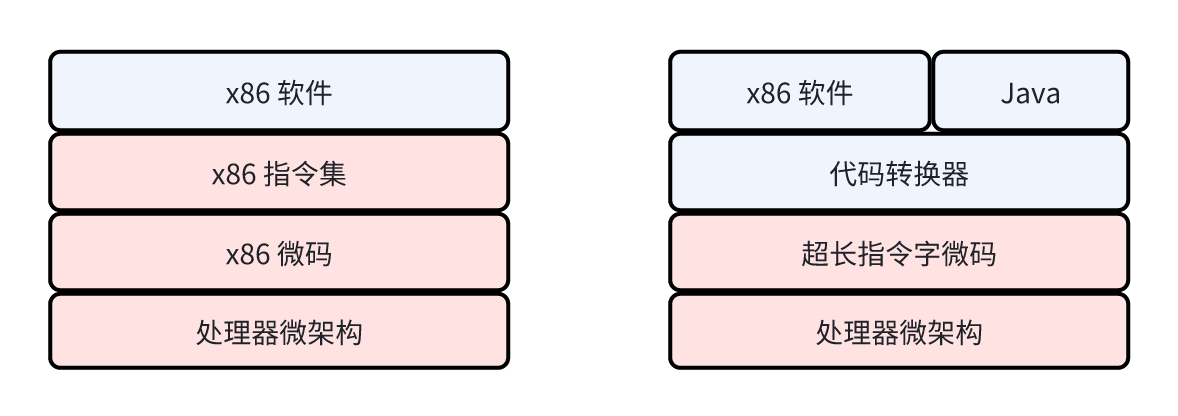
\includegraphics[width=0.8\linewidth]{./feishuImage/transmeta_arch.png}
    \caption{全美达架构图,在超长指令字处理器上实现兼容X86的指令集,并支持JAVA程序。}
    \label{img:transmeta_arch}
  \end{figure}


由于目前超标量乱序处理器的硬件乱序调度已经十分成熟,超长指令字设计在通用处理器上的流行度已经减弱,但 全美达 公司的工作为多架构兼容性提供了有益的经验。

\subsection{纯软件二进制翻译器的相关工作}

在纯软件领域,用户态二进制翻译器扮演着重要的角色。QEMU 是一款广泛使用的开源模拟器,支持多种指令集架构。如图\ref{img:qemu_arch},其核心目标之一是提供多架构的虚拟化支持,使用户能够在不同的硬件平台上运行其应用程序。它通过将不同指令集的机器代码翻译成中间语言(IR,Intermediate Representation),再将IR翻译成宿主指令集,实现跨架构的兼容性。这种设计使得QEMU能够处理多种指令集,为用户提供了一定的灵活性。然而,QEMU的性能仅能达到原生性能的13\%,这主要归因于双层翻译的性能损失。

\begin{figure}[h]
  \centering
  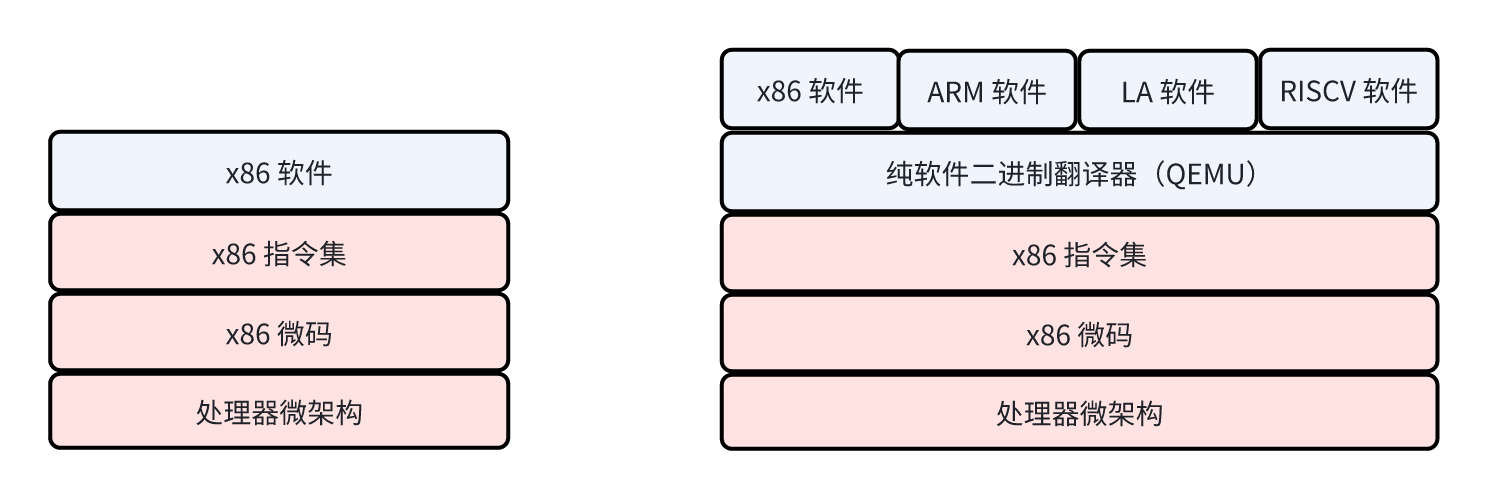
\includegraphics[width=0.8\linewidth]{./feishuImage/qemu_arch.png}
  \caption{QEMU二进制翻译器架构图,能在宿主指令集机器上运行多种客户程序。}
  \label{img:qemu_arch}
\end{figure}

尽管QEMU在实现多架构支持上取得了一些成功,但在性能方面仍然面临挑战。其性能仅相当于原生性能的一小部分,这在一些对性能要求较高的应用场景下显得不够可用。

其他常用的商用级用户级二进制翻译器,参见表\ref{tab:BTs},例如苹果公司的Rosetta2(67.2\%)、华为公司的ExaGear(72.7\%)、龙芯公司的LATX(60\%)等,性能上仍然无法接近原生性能。这些二进制翻译器采用一对一指令的翻译方式,即把一种指令集直接翻译到另一种指令集上(但一条客户指令可能翻译成多条宿主指令,产生指令膨胀,导致性能下降)。它们虽然在理论上支持多架构翻译,但实际上需要投入较大的工程量,也可能造成性能下降。

\begin{table}[]
\centering
\caption{主流二进制翻译器}
\label{tab:BTs}
  \begin{tabular}{llll}
  \rowcolor[HTML]{FBE5D6} 
  二进制翻译器    & 公司   & 客户平台           & 宿主平台           \\
  ExaGear   & 华为   & X86            & ARM            \\
  Rosetta2  & 苹果   & X86            & ARM            \\
  LoongArch & 龙芯   & X86            & LoongArch      \\
  QEMU      & 开源项目 & X86,ARM,RISCV等 & X86,ARM,RISCV等
  \end{tabular}
  \end{table}

\subsection{软件二进制翻译的性能开销来源}

\begin{figure}[h]
  \centering
  \includegraphics[width=1\linewidth]{./plot/insts_inflt_breakdown_2017.pdf}
  \caption{QEMU二进制翻译器架构图,能在宿主指令集机器上运行多种客户程序。}
  \label{img:insts_inflt_breakdown_2017}
\end{figure}

根据我们之前完成的一项工作,使用指令膨胀率来分析二进制翻译器的性能开销。指令膨胀率是指,每条客户指令平均翻译出的宿主指令数,是一个大于1的小数,计算方式为$\mbox{总体膨胀} = \mbox{生成的宿主指令数} / \mbox{客户指令数}$(这里用的是动态运行指令数)。指令膨胀率越高,翻译后的程序要执行的指令数越多,执行时间越长,性能越低。如图\ref{img:insts_inflt_breakdown_2017},我们主要把开销分成了5类:

%latex 使用1. 2. 3. 来编号
\begin{enumerate}
  \item \textbf{指令集间操作码差异:} 不同指令集的操作码差异引起Eflags计算等操作的额外指令翻译,增加了指令膨胀率。此外LoongArch对于子寄存器默认符号扩展,X86/ARM默认零扩展。对应图\ref{img:insts_inflt_breakdown_2017}中\textcolor{brown}{棕色}部分。
  
  \item \textbf{操作数据模式不同:} 复杂指令集(如X86)可以直接访问内存,而其他精简指令集只能操作寄存器,导致操作数模式不同。对应图\ref{img:insts_inflt_breakdown_2017}中\textcolor{orange}{橙色}部分。
  
  \item \textbf{地址计算不同:} 复杂地址计算方式(如X86)与其他指令集的简单计算方式导致在翻译时需要额外指令。例如X86计算地址$addr = base + index * scale +disp$; 其他的大多为$addr = base + offset$。 对应图\ref{img:insts_inflt_breakdown_2017}中\textcolor{green}{绿色}部分。
  
  \item \textbf{立即数加载:} X86支持编码64位立即数和32位地址偏移,而其他指令集编码空间有限,导致立即数加载的语义不同,需要额外的访存指令或者是多条立即数加载指令。对应图\ref{img:insts_inflt_breakdown_2017}中\textcolor{red}{红色}部分。
  
  \item \textbf{间接跳转:} 客户指令地址到宿主指令地址是非线性的,而间接跳转的目标地址在运行时才能知道,需要查询间接跳转哈希表,导致性能开销。对应图\ref{img:insts_inflt_breakdown_2017}中\textcolor{purple}{紫色}部分。
  
\end{enumerate}

以上这5类主要开销很难通过软件优化来解决,需要借助硬件辅助的方式来解决。

为了消除软件二进制翻译器的性能开销,特别是在处理指令集语义差异方面的挑战,本文采用了硬件辅助的策略。其中,一些关键的工作包括:

1. 融合微码以缩小指令集语义差距: 针对指令集间操作码差异、操作数据模式不同以及地址计算不同等问题,我们尝试通过融合微码的方式,减小不同指令集之间的语义差距,从而降低翻译的开销。

2. 微码缓存的思路应用: 针对立即数加载和间接跳转的性能开销,我们借鉴了X86微码缓存的思想,将立即数放入微码缓存行中直接加载,用微码缓存直接查询非线性的地址空间映射,消除这两类开销。

接下来,将介绍与X86微码缓存相关的工作,探讨如何借助硬件辅助手段进一步优化软件二进制翻译器的性能。


\subsection{X86 微码缓存的相关工作}

X86 微码缓存是为了在 X86 CPU 后端实现超标量乱序执行而引入的关键组件,如图\ref{img:front_end_ucache}。以下是关于 X86 微码缓存的主要工作和设计特点:

\begin{figure}[h]
  \centering
  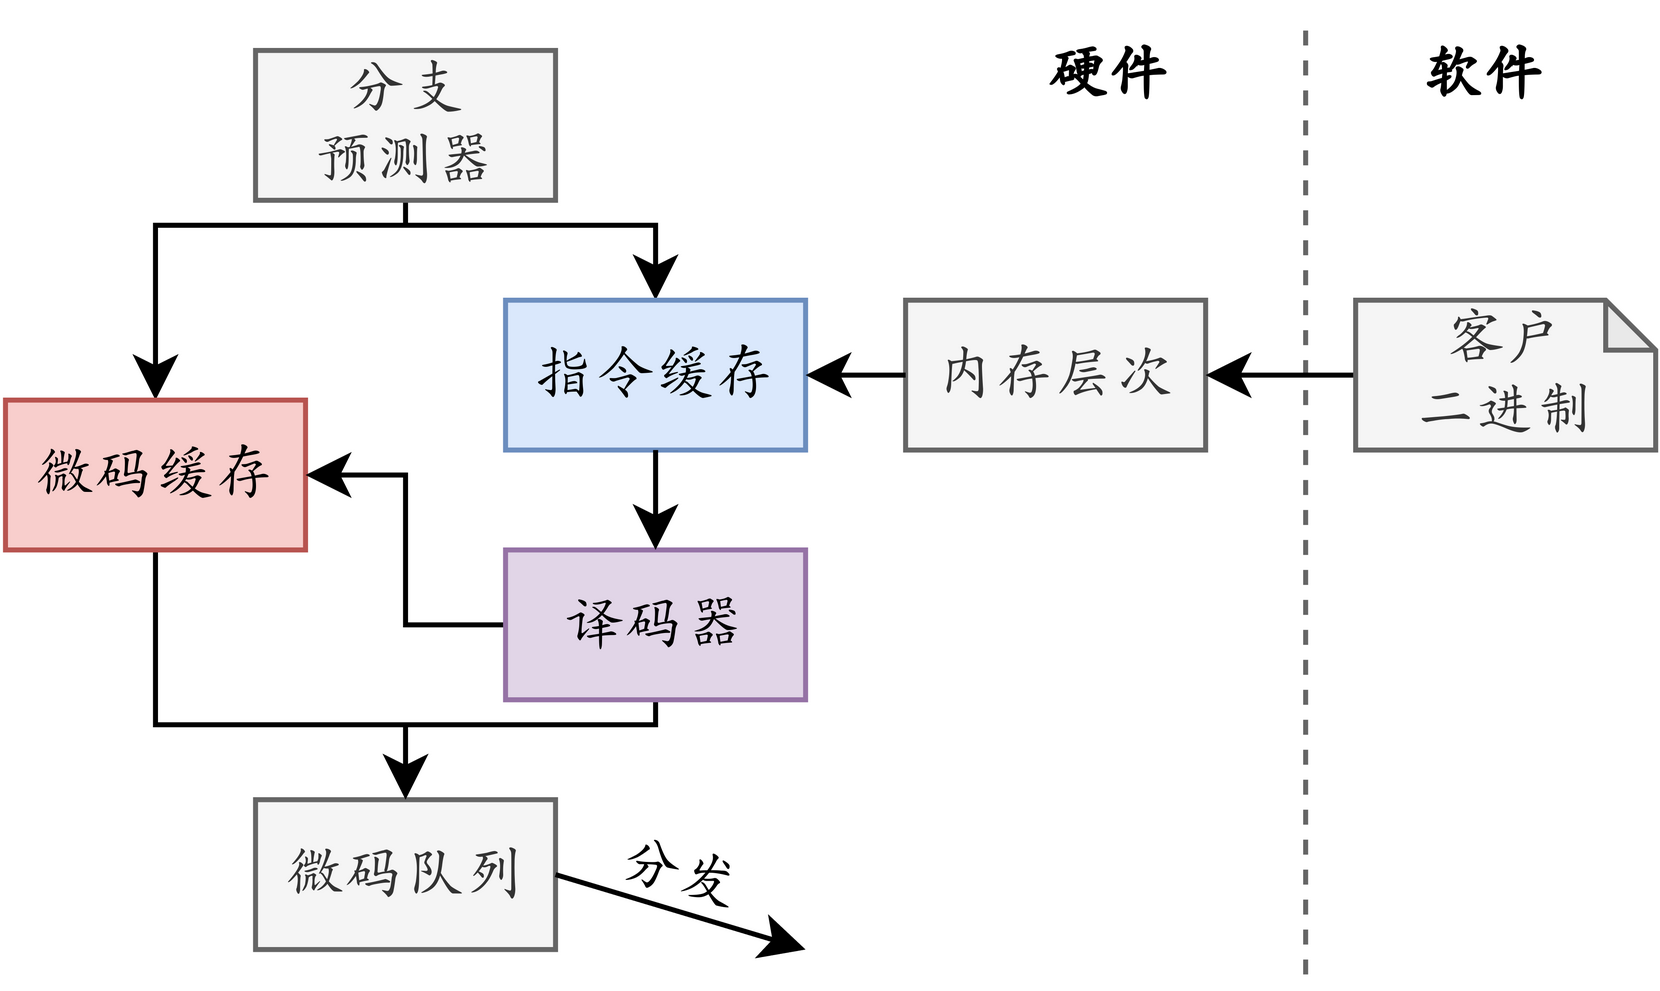
\includegraphics[width=0.8\linewidth]{./image/front_end_ucache.pdf}
  \caption{X86处理器前端架构图,包括指令缓存和微码缓存}
  \label{img:front_end_ucache}
\end{figure}

\begin{figure}[h]
  \centering
  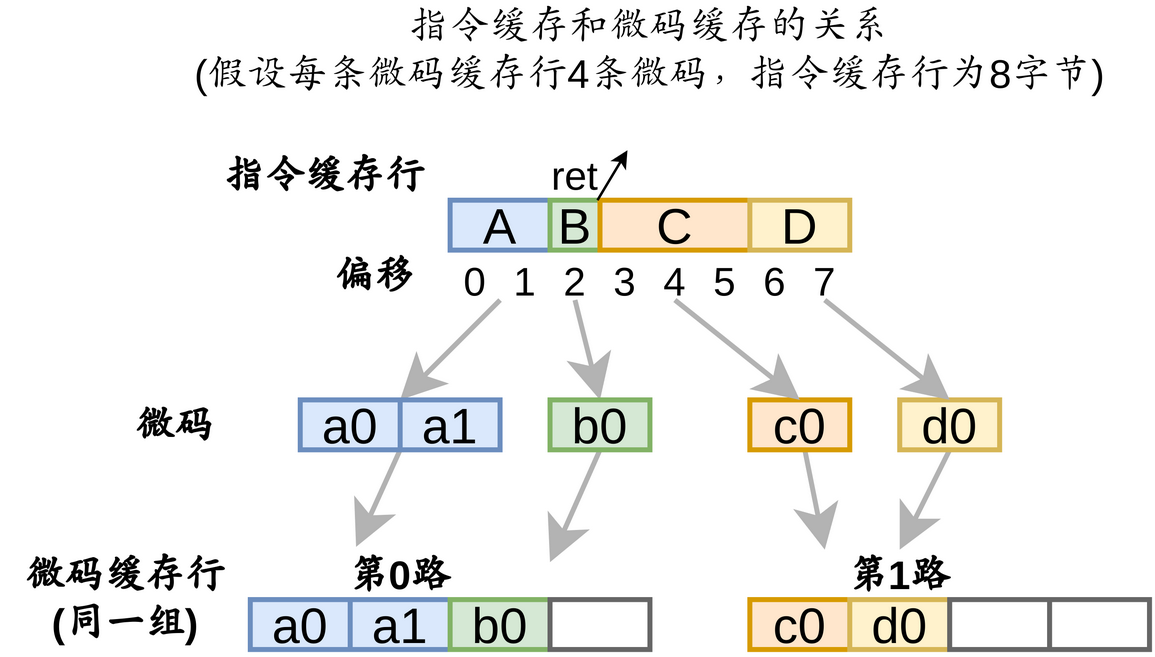
\includegraphics[width=0.8\linewidth]{./image/IC-to-UC.pdf}
  \caption{指令缓存和微码缓存关系}
  \label{img:IC_to_UC}
\end{figure}

1. \textbf{微码与超标量乱序执行的关系:}

   - 为了实现超标量乱序执行,X86 CPU 后端需要将复杂指令译码为简单指令,即微码。

   - 微码的引入简化了指令集的关系,使得 CPU 在后端能够更高效地执行。

2. \textbf{微码缓存的引入:}

- 为了降低译码能耗、提高性能,研究者们引入了微码缓存,用于存储已经译码过的微码。

- 微码缓存的设计目的是减少译码的重复计算,从而提高整体指令执行效率。

3. \textbf{查询与缓存机制:}
  
- 在前端译码阶段,系统首先查询微码缓存,检查是否已经缓存了当前指令的微码。

- 如果微码已经在缓存中,CPU 就直接读取微码并发射到后端执行。

- 如果微码未缓存,系统则从指令缓存中取得指令,进行译码,并将译码结果存入微码缓存中,见图\ref{img:IC_to_UC},注意一个指令缓存行可能生成多个微码缓存行。

4. \textbf{缓存组织形式:}

- 微码缓存的组织形式与指令缓存有所区别。它以第一条指令的程序计数器(PC)作为索引,来索引整行的微码。

- 当遇到控制流指令时,微码缓存会截断这一行,确保每个缓存行只包含一个基本块的微码,参考图\ref{img:IC_to_UC}中的ret指令。

- 微码行中除了存入微码外,还会在最后存储立即数,见图\ref{img:ucache_line},这是由于X86是变长指令集,微码是定长指令集,遇到长立即数时候就会放在微码行最后。

X86 微码缓存的引入和优化为 X86 架构的超标量乱序执行提供了重要支持,使得 CPU 在执行 X86 指令集时能够更加高效地利用硬件资源,提高整体性能。

\begin{figure}[h]
  \centering
  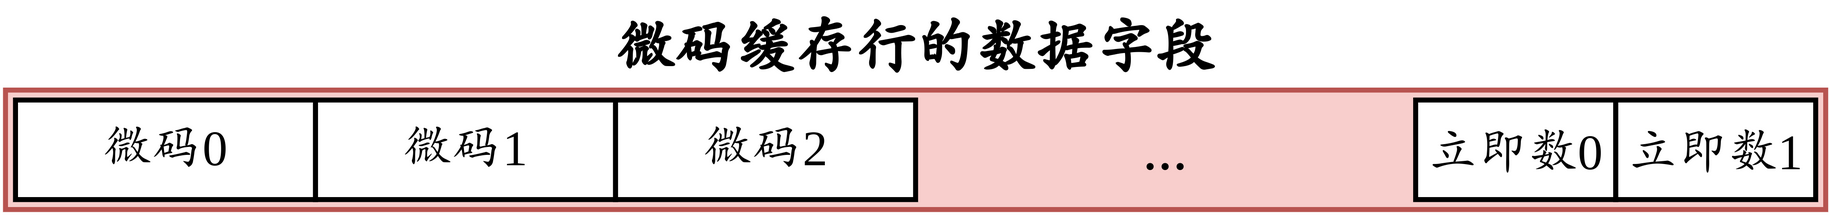
\includegraphics[width=0.8\linewidth]{./image/ucache_line.pdf}
  \caption{指令缓存和微码缓存关系}
  \label{img:ucache_line}
\end{figure}

%---------------------------------------------------------------------------%
%->> Chapter 3
%---------------------------------------------------------------------------%

\section{课题主要研究内容、预期目标}


\begin{figure}[h]
  \centering
  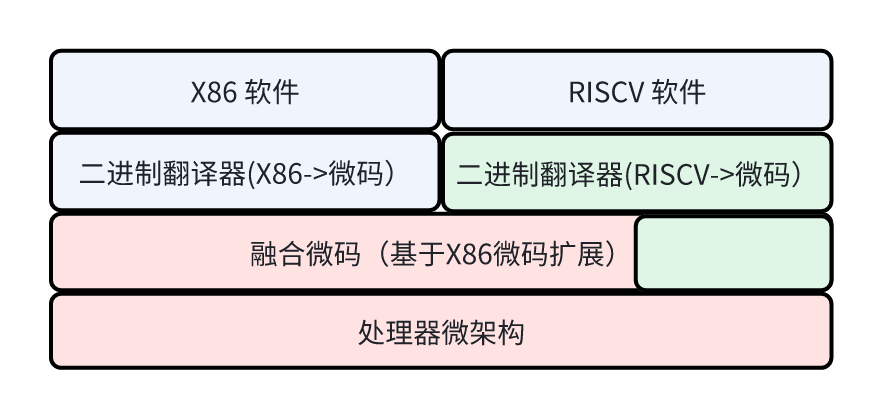
\includegraphics[width=0.8\linewidth]{./feishuImage/implement_arch.png}
  \caption{多架构软硬协同的二进制翻译架构实现图,绿色部分为本文主要工作。}
  \label{img:implement_arch}
\end{figure}

本课题旨在解决\textbf{多架构指令集兼容问题}和\textbf{传统二进制翻译器的性能瓶颈},通过引入微译器的概念,结合软硬协同的思想,以及借鉴微码缓存和微码指令集的理念,从软硬件两个层面进行优化。

本课题旨在探索多架构的可行性,所以仅实现X86和RISCV的二进制翻译。但是本课题的设计思想可以推广到其他指令集架构上。

\subsection{整体架构}
1. 如图\ref{img:implement_arch},整体上,硬件层仅对外暴露融合微码,软件层面的二进制翻译器可以实现多架构的支持。这一步旨在提高软件层面的二进制翻译器的性能,降低软件层面的性能瓶颈。

2. 在软件层面,将在已有X86二进制翻译的模式下,添加 RISCV 版本的二进制翻译器。这一步旨在验证多架构的可行性,以及提高软件层面的二进制翻译器的性能。

3. 在硬件层面,将在已有X86微码的模式下,添加必要的类RISCV微码,实现融合微码的硬件设计,力求实现RISCV到微码的一对一的指令翻译,以降低指令膨胀率。这一步旨在提高硬件执行效率,减小性能开销。


%---------------------------------------------------------------------------%
%->> Chapter 4
%---------------------------------------------------------------------------%


\section{拟采用的研究方法、技术路线、实验方案及其可行性分析}

\begin{figure}[h]
  \centering
  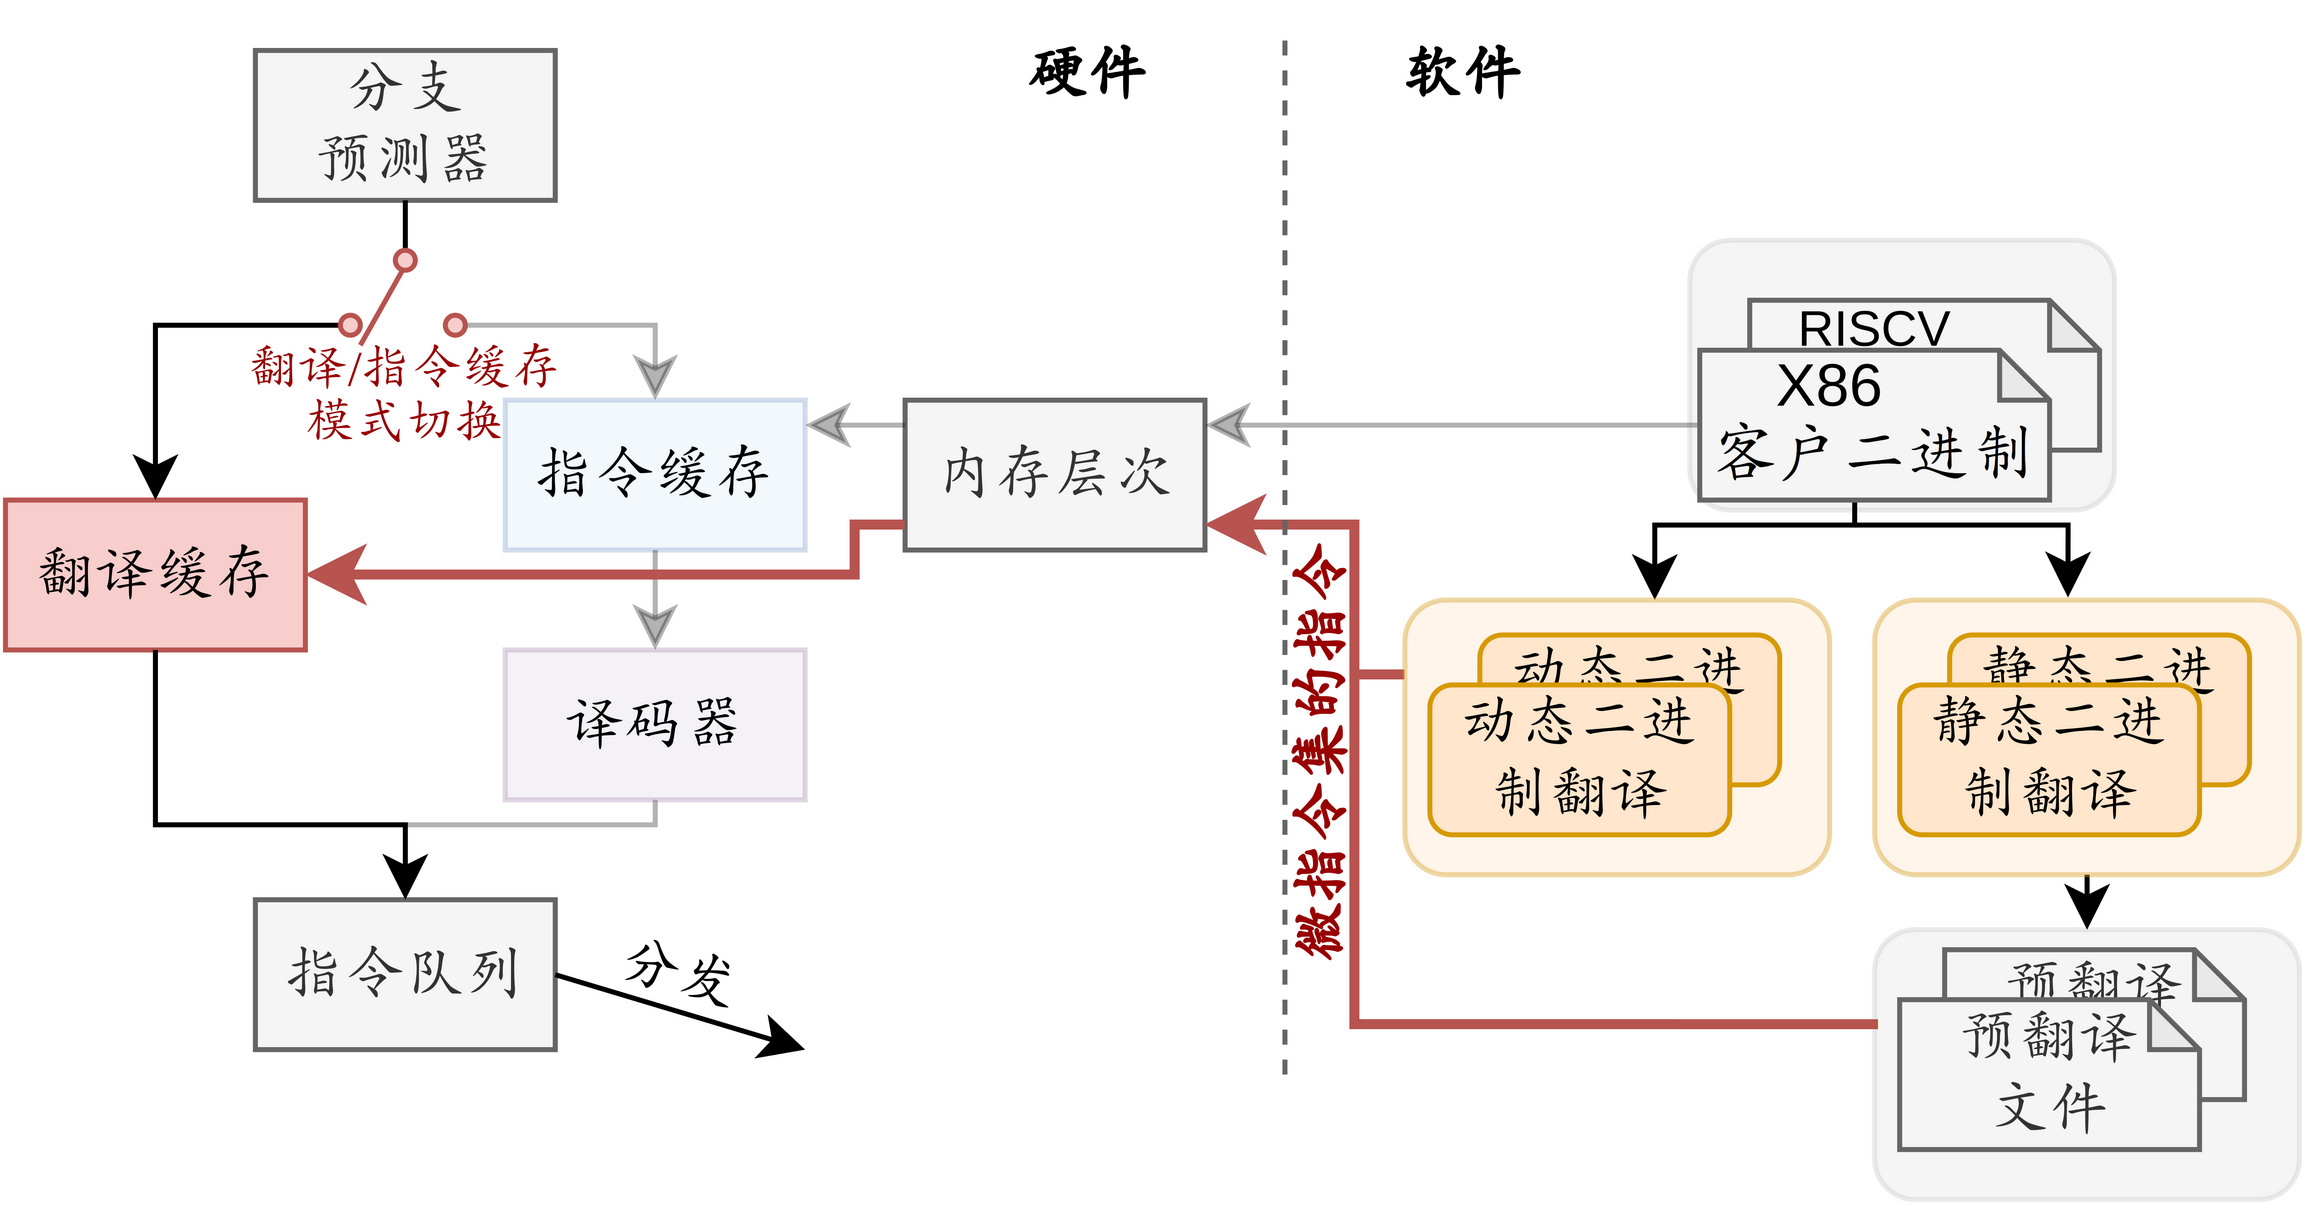
\includegraphics[width=1\linewidth]{./image/front_end_transutor.pdf}
  \caption{架构细节图。}
  \label{img:front_end_transutor}
\end{figure}

\subsection{微译器架构细节}

为了解决传统二进制翻译的性能瓶颈,本课题在已有的微译器的概念下,添加RISCV多架构支持。首先介绍微译器的架构细节,如图\ref{img:front_end_transutor}:

\subsubsection{硬件部分}

在硬件部分,引入了翻译缓存(Translation Cache),该缓存作为一级缓存负责存储预翻译的微码指令集,替代了原本的微码缓存。与传统微码架构不同,翻译缓存通过二进制翻译透过内存层次(从内存加载到L3 Cache, 再到L2Cache, 最后到微码缓存)进行填充,取代了传统的指令缓存和译码器的角色。在传统X86架构下,取指部件会同时查询指令缓存和微码缓存;而在微译器架构下,取指部件仅查询翻译缓存,硬件的译码器被软件的二进制翻译器取代。

\subsubsection{软件部分}

在软件部分,引入了静态和动态二进制翻译器。程序首先通过静态二进制翻译器被翻译成微指令,并被写入预翻译文件,存储在硬盘中。在客户程序执行阶段,预翻译文件被加载到内存中,程序计数器被设置为客户程序的入口。取指部件从翻译缓存中取指,若翻译缓存或内存层次命中,则与从指令缓存取指类似,不断取指执行。若翻译缓存和内存层次均未命中(例如存在自修改代码等),说明客户指令还未翻译,此时会调用动态二进制翻译器进行实时翻译。


\subsection{RISCV多架构支持}

1. 在硬件层面,将在已有X86微码的模式下,力求实现RISCV到微码的一对一的指令翻译,以降低指令膨胀率。为此需要添加必要的类RISCV微码,包括编码设计,后端微码执行逻辑设计,压缩指令设计等。

2. 在软件层面,将在已有X86二进制翻译的模式下,添加 RISCV 版本的二进制翻译器。需要添加RISCV到微码的翻译规则,寄存器映射规则,压缩指令的翻译规则等。


\subsection{实验环境}

为了全面评估微译器的性能和效果,我们实现了以下硬件和软件模块:

\subsubsection{硬件环境}

\begin{itemize}
  \item \textbf{Gem5 模拟器:} 我们在 Gem5 模拟器\cite{Gem5SimulatorVersion2020}上实现了微译器的硬件原型系统。Gem5 提供了一个灵活且可配置的模拟环境,能够模拟多种体系结构和处理器类型。

  \item \textbf{处理器模型:} 我们选择了 X86 Haswell\cite{akramValidationGem5Simulator2019} 校准过的 V23 最新版本。为了模拟真实硬件环境,我们采用了乱序处理器模型(DeriveO3CPU),

  \item \textbf{硬件配置:} 实验中,我们保持硬件配置与原本的 X86 CPU 一致,唯一的区别是将代码缓存替换为翻译缓存,以验证微译器的性能。
\end{itemize}

\subsubsection{软件环境}

\begin{itemize}
  \item \textbf{二进制翻译器:} 我们复用了部分LLVM objdump\cite{llvm_project}的代码发现逻辑,使用了Capstone\cite{CapstoneEngine2023}作为反汇编器(LLVM 和Capstone都支持多指令集,也方便后续添加新的指令集支持),并添加好翻译规则,实现了静态二进制翻译器,每个翻译器代码量级仅在千行。由于SPEC CPU 2017 不存在代码发现问题,目前尚未实现动态二进制翻译器。

  \item \textbf{SimPoint 技术:} 由于Gem5的模拟执行效率约为真机的万分之一,为了更快速有效地进行性能评估,我们使用 SimPoint技术\cite{sherwoodAutomaticallyCharacterizingLarge2002} 对 SPEC CPU 2017 进行切片,使用ELFie技术\cite{patilELFiesExecutableRegion2021}对二进制文件进行切片,以提高模拟效率。
\end{itemize}



\section{已有科研基础与所需的科研条件}

本章节首先展示微译器在X86上SPEC 2017上的翻译运行结果,然后介绍RISCV在CoreMark测试集上的运行效果。

\subsection{微译器在X86上的翻译运行结果}

图\ref{img:ucache_ipc}展示了微译器在X86上SPEC 2017上的翻译运行结果,相对于未修改过的X86指令缓存模式进行了归一化。可以看到,微译器在SPEC 2017上的性能接近于原生运行,平均性能为92.3\%,并且一大半的浮点型测试集的性能损失在1\%以内。

\begin{figure}[h]
  \centering
  \includegraphics[width=1\linewidth]{./plot/ucache_ipc.pdf}
  \caption{微译器运行SPEC CPU 2017的性能,相对于未修改过的X86指令缓存模式进行了归一化。}
  \label{img:ucache_ipc}
\end{figure}

图\ref{img:new_cache_miss}展示了微译器在X86上SPEC 2017上的每千条指令的未命中次数,根据计算,每千条指令的未命中次数和性能之间的皮尔森相关系数为-0.93,说明未命中次数和性能之间存在很强的负相关性。这也说明了微译器的性能主要受到了未命中次数的影响。

我们在X86上运行了CoreMark测试集,得到了性能为99\%,对应的每千条指令的未命中次数为0.9,也符合上述规律,这主要在于程序的取指行为,CoreMark程序中主要为核心循环计算,时间局部性和空间局部性都很好,因此未命中次数较少,性能也较好。即便经过微译器的预翻译文件膨胀,也能够在X86上保持较好的性能。

\begin{figure}[h]
  \centering
  \includegraphics[width=1\linewidth]{./plot/new_cache_miss.pdf}
  \caption{微译器运行SPEC CPU 2017的每千条指令的未命中次数。}
  \label{img:new_cache_miss}
\end{figure}

\subsection{RISCV在CoreMark测试集上的运行效果}

我们在RISCV上运行了CoreMark测试集,得到了性能为95\%,对应的每千条指令的未命中次数为1.1,也符合上述规律。

RISCV 相对于X86的CoreMark 还有一定的性能差距,主要由于还没有添加硬件返回栈支持,导致对于函数调用的支持不够完善,因此性能有所下降。

同时RISCV目前对于压缩指令支持还不够完善,导致翻译出来的微码编码较长,导致AOT文件相对更大,也会导致性能下降。

\section{研究工作计划与进度安排}

以下为本课题的工作计划与进度安排:

\begin{itemize}
  \item 2023年12月-2023年12月:添加RISCV硬件返回栈支持,预估有5\%左右性能提升。
  \item 2023年12月-2024年2月:继续添加完所有的指令翻译和微码添加,目标为成功运行SPEC CPU 2000。
  \item 2024年2月-2024年3月:RISCV 到微码的指令编码继续压缩,减少每条指令平均长度。
  \item 2024年3月-2024年4月:撰写硕士毕业论文。
\end{itemize}


% \nocite{*}% 使文献列表显示所有参考文献(包括未引用文献)
%---------------------------------------------------------------------------%



%-
%-> Backmatter: bibliography, glossary, index
%-
\artxifstreq{\artxbib}{bibtex}{% enable bibtex
    \bibliography{./kaiti.bib}% bibliography
}{%
    \printbibliography% bibliography
}
\end{document}
%---------------------------------------------------------------------------%

